\chapter{Schleifen}
\label{chp:loops}
\epigraph{
	Insanity: doing the same thing over and over again and expecting different results
}{Albert Einstein}

Computer können dazu benutzt werden, die immer gleichen (lästigen) Aufgaben wiederholt und in schneller Folge auszuführen. Es ist möglich, bei jeder Wiederholung einen einzelnen Eingabewert zu ändern und so \eg Berechnungen für einen ganzen Wertebereich durchzuführen, oder Messwerte von einem Gerät zu überwachen.

Zeichnet man ein \emph{Flussdiagramm} eines solchen Programms (wie in Abbildung \ref{fig:FlowBasicLoop}), so findet sich in der Regel ein Programmteil, der zur Vorbereitung dient und in gewohnter Weise \enquote{von oben nach unten} abgearbeitet wird. An diesen schließt sich ein Abschnitt an, der einige Male wiederholt werden soll, und daher im Flussdiagramm als Bogen dargestellt wird. Nach diesem Teil könnte die Ausgabe der Ergebnisse stattfinden, die wiederum in gewohnter \emph{linearer} Weise (also von oben nach unten) bearbeitet wird. 

Die Form dieses Flussdiagramms motiviert den Namen \emph{Schleife} für eine solche Struktur.

\begin{figure}[h!]
\begin{center}
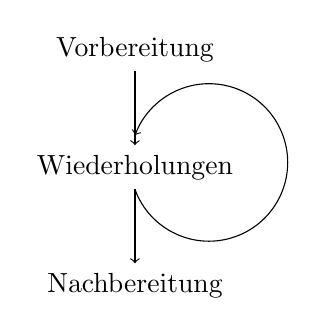
\begin{tikzpicture}
    \node at (0, 3  ) (Input)      {Vorbereitung};
    \node at (0, 1.5) (Operations) {Wiederholungen};
    \node at (0, 0  ) (Output)     {Nachbereitung};
    
    \draw [->] (Input) -- (Operations);
    \draw [->] (Operations.south)arc(-160:160:1.0);		%start angle: stop angle : radius
    \draw [->] (Operations) -- (Output);
\end{tikzpicture}
\caption{Programmflussdiagramm mit Schleife} \label{fig:FlowBasicLoop}
\end{center}
\end{figure}

In der Regel ist die Zahl der Schleifendurchläufe an eine Bedingung geknüpft; genauso sind aber auch \emph{Endlosschleifen} möglich. In diesem Kapitel werden wir verschiedene Schleifentypen und ihre Anwendungsfelder kennen lernen.

\begin{hintbox}[Laufende Programme zum Beenden zwingen: \texttt{STRG + C}]
Macht man einen Fehler bei der Formulierung der Bedingung, so kann man unbeabsichtigt eine Endlosschleife erstellen. Ein solches Programm wird von sich selbst aus nie beendet. Wir können zu jeder Zeit aber das Beenden erzwingen, indem wir in der Konsole die Tastenkombination \texttt{STRG + C} drücken.
\end{hintbox}

\section{\inPy{while}-Loops}
\subsection{Grundstruktur}
Mit dem Schlüsselwort \inPy{while} wird ein Codeblock eingeleitet, der so lange wiederholt wird, bis eine Bedingung nicht mehr erfüllt ist, \ie bis ihr Wahrheitswert zu \inPy{False} ausgewertet wird. Die Syntax lautet:

\begin{codebox}[Syntax: \texttt{while} (1)]
\begin{minted}{python}
while Wahrheitswert :
    Schleifenkoerper
\end{minted}
\end{codebox}

Betrachten Sie hierzu folgendes Beispiel zum Zinseszins: \enquote{berechnet} wird, nach wie vielen Jahren ein Startkapital bei gegebenem Zinssatz über einen Grenzwert hinauswächst\footnote{Natürlich ließe sich dies auch über die Logarithmus-Funktion realisieren; hier aber soll die Funktionsweise von Schleifen gezeigt werden}.

\begin{codebox}[Beispiel: Zinseszins (1)]
\begin{minted}[linenos]{python}
capital  = float(input("Bitte geben Sie Ihr Startkapital ein: "))
interest = float(input("Bitte geben Sie den Zinssatz ein: "    ))
limit    = float(input("Bitte geben Sie Ihr Zielkapital ein :" ))

years    = 0

while capital < limit :
    capital *= 1 + interest
    years   += 1

print("Nach", years, "Jahren ist das Sparziel erreicht.")
\end{minted}
\end{codebox}

Nachdem die Variablen \inPy{capital, interest, limit} und \inPy{years} ihre Werte zugewiesen bekommen haben, wird überprüft, ob \inPy{capital < limit}. Wenn dies erfüllt ist, werden die Zeilen 8 und 9 ausgeführt. Danach springt die Codeausführung zurück zu Zeile 7. Es wird solange der Schleifenkörper in Zeile 8 und 9 wiederholt, bis die Bedingung in Zeile 7 nicht mehr erfüllt ist. Erst dann wird mit der Ausführung in Zeile 11 fortgesetzt. So erklärt sich folgendes Ausführungsbeispiel:

\begin{cmdbox}[Ausführungsbeispiel: Zinseszins (1)]
\begin{minted}{text}
Bitte geben Sie Ihr Startkapital ein: 100
Bitte geben Sie den Zinssatz ein: .1
Bitte geben Sie Ihr Zielkapital ein :300
Nach 12 Jahren ist das Sparziel erreicht.
\end{minted}
\end{cmdbox}

Der Schleifenkörper wird nie ausgeführt, wenn die Bedingung nicht bereits vor Beginn der Schleife erfüllt war. Geben Sie im obigen Beispiel etwa ein Startkapital ein, das größer als das Zielkaptital ist, so folgt die Ausgabe \texttt{Nach 0 Jahren ist das Sparziel erreicht.} Die Zeile \inPy{years += 1} wird nie ausgeführt.

\begin{hintbox}[Endlosschleifen]
Manchmal möchte man, dass ein Programm auf unbestimmte Zeit läuft. Code, der die Messwerte einer Wetterstation verarbeitet, soll dies vielleicth \enquote{für immer} tun. In diesem Fall bietet sich eine Endlosschleife an:
\end{hintbox}
\begin{hintbox}[]
\begin{codebox}[Code: Endlosschleife]
\begin{minted}[linenos]{python}
while True:
  Anweisungen
\end{minted}
\end{codebox}
Da \inPy{True} eine Konstante ist, wird sich nichts daran ändern, dass sie immer eben zu \inPy{True} ausgewertet wird. Das Programm läuft bis in alle Ewigkeiten (oder zumindest, bis es vom Betriebssystem beendet wird). Üblicherweise enthält \inPy{Anweisungen} dann Code, der das Programm dennoch zu einem Ende führt. Diese Anweisungen könnten aber an komplexe Bedingungen geknüpft sein, die für die Form von \inPy{while} zu sperrig sind.
\end{hintbox}


\subsection{Eingriff in den Kontrollfluss}
Es gibt Situtaionen, wo die Ausführung einer Schleife an mehrere, voneinander unabhängige Bedingungen geknüpft sind. Dies lässt sich mit logischen Operatoren (Siehe Abschnitt \ref{sec:Booleans}) umsetzen. Häufig ist es aber übersichtlicher, das Schlüsselwort \inPy{break} in einem eigenen \inPy{if}-Block zu benutzen. Mit \inPy{break} wird der Schleifenkörper verlassen, die Ausführung wird hinter der Schleife fortgesetzt, ganz als ob die Bedingung hinter \inPy{while} selbst nicht mehr erfüllt wäre. Zusätzlich zur Übersichtlichkeit bietet diese \inPy{break}-Methode die Möglichkeit, an einem beliebigen Punkt innerhalb der Schleife zu prüfen, ob der Schleifenkörper verlassen werden soll.

\begin{codebox}[Beispiel: \texttt{break}]
\begin{minted}[linenos]{python}
count = 0
value = 0

while count < 12 :
    newValue = float(input("Bitte geben Sie einen weiteren Wert ein: "))
    value += newValue
    count += 1
  
    if value > 9000 :
        value = "over nine thousand!!"
        break
  
    print(
        "Bisheriger Gesamtwert nach Eingabe von", count, 
        "Werten:", value
    )

print("Gesamtwert:", value)
\end{minted}
\end{codebox}

Das Einlesen von \inPy{newValue} sowie die Updates an \inPy{value} und \inPy{count} werden bei jedem Durchlauf der Schleife durchgeführt. Die Ausgabe des Zwischenstandes (Zeilen 13-16) hingegen nur, wenn die Zweite Bedingung (\inPy{value > 9000}) nicht erfüllt war. So erklärt sich folgendes Ausführungsbeispiel:

\begin{cmdbox}[Ausführungsbeispiel: \texttt{break}]
\begin{minted}{text}
Bitte geben Sie einen weiteren Wert ein: 1
Bisheriger Gesamtwert nach Eingabe von 1 Werten: 1.0
Bitte geben Sie einen weiteren Wert ein: 50
Bisheriger Gesamtwert nach Eingabe von 2 Werten: 51.0
Bitte geben Sie einen weiteren Wert ein: 9000
Gesamtwert: over nine thousand!!
\end{minted}
\end{cmdbox}

Ähnlich kann \inPy{continue} benutzt werden, um einen Teil des Schleifenkörpers zu überspringen, ohne die Schleife selbst zu verlassen. Der Befehl \inPy{continue} springt also zur Überprüfung der \inPy{while}-Bedingung zurück:

\begin{codebox}[Beispiel: \texttt{continue}]
\begin{minted}[linenos]{python}
container = []

while len(container) < 3 :
    value = int(input("Bitte geben Sie eine gerade Zahl ein: "))
  
    if value % 2 :
        print(value, "ist ungerade und daher nicht zulässig.")
        continue
  
    container.append(value)
    print("Bisher eingegeben: ", container)
\end{minted}
\end{codebox}

\begin{cmdbox}[Ausführungsbeispiel: \texttt{continue}]
\begin{minted}{text}
Bitte geben Sie eine gerade Zahl ein: 2
Bisher eingegeben:  [2]
Bitte geben Sie eine gerade Zahl ein: 3
3 ist ungerade und daher nicht zulässig.
Bitte geben Sie eine gerade Zahl ein: 4
Bisher eingegeben:  [2, 4]
Bitte geben Sie eine gerade Zahl ein: 6
Bisher eingegeben:  [2, 4, 6]
\end{minted}
\end{cmdbox}

\begin{hintbox}[Garantierte erste Ausführung]
Wir können Endlosschleifen zusammen mit \inPy{break} nutzen, um zu garantieren, dass der Schleifenkörper mindestens einmal ausgeführt wird, unabhängig davon, ob die Schleifenbedingung zu Anfang bereits erfüllt war:
\begin{codebox}[Beispiel: \texttt{continue}]
\begin{minted}[linenos]{python}
while True:
    Schleifenkoerper
    if Bedingung :
        break
\end{minted}
\end{codebox}
Die Überprüfung auf \inPy{Bedingung} wird so an das Schleifenende geschoben.
\end{hintbox}


\subsection{\texttt{else} bei \texttt{while}}
Wie schon angesprochen wird der Schleifenkörper nicht ausgeführt, wenn die Bedingung schon vor der ersten Durchführung nicht erfüllt war. In diesem Fall kann ein optionaler \inPy{else}-Block ausgeführt werden:

\begin{codebox}[Syntax: \texttt{while} (2)]
\begin{minted}{python}
while Wahrheitswert :
    Schleifenkoerper
else :
    AlternativCode
\end{minted}
\end{codebox}

Betrachten wir dies an einem erweiterten Beispiel:
\begin{codebox}[Beispiel: Zinseszins (2)]
\begin{minted}[linenos]{python}
capital  = float(input("Bitte geben Sie Ihr Startkapital ein: "))
interest = float(input("Bitte geben Sie den Zinssatz ein: "    ))
limit    = float(input("Bitte geben Sie Ihr Zielkapital ein :" ))

years    = 0

while capital < limit :
    capital *= 1 + interest
    years   += 1
else :
    print("Das Startkapital ist bereits groß genug.")
  
print("Nach", years, "Jahren ist das Sparziel erreicht.")
\end{minted}
\end{codebox}

Die Zeile \texttt{Das Startkapital ist bereits groß genug.} wird genau dann ausgegeben, wenn für \inPy{capital} ein Wert größer oder gleich \inPy{limit} eingegeben wurde. Weiterhin wird für diesen Fall \texttt{Nach 0 Jahren ist das Sparziel erreicht.} als zweite Zeile ausgegeben.

\begin{warnbox}[Garantierte erste Ausführung mit \texttt{else}]
Statt der oben gezeigten Form mit \inPy{break} könnte auch mit \inPy{else} dafür gesorgt werden, dass der Schleifenkörper mindestens einmal ausgeführt wird. Hierzu kopiert man einfach den kompletten Code des Schleifenkörpers in den \inPy{else}-Block.

Dies erfüllt zwar seinen Zweck, ist aber eine Fehlerquelle und sollte vermieden werden. Wenn Sie später Codestellen ändern, müssen Sie auch daran denken, dieselben Änderungen im \inPy{else}-Block umzusetzen. Dies wird leicht vergessen.
\end{warnbox}

    
\section{\inPy{for}-Loops}
\subsection{Grundstruktur}
Schleifen mit \inPy{for} führen Code für jedes Element aus einer Datenstruktur wie in Kapitel \ref{chp:Containers} beschrieben aus. Nacheinander wird jedes Element des Containers über eine Hilfsvariable ansprechbar gemacht und dann Code ausgeführt, der von dieser Hilfsvariablen abhängig sein kann.

\begin{codebox}[Syntax: \texttt{for}]
\begin{minted}{python}
for Variable in Container :
    Schleifenkoerper
\end{minted}
\end{codebox}

Der Code lässt sich also fast wie englische Sprache lesen: \enquote{für jedes Objekt in \emph{Container} mache \emph{Schleifenkörper}}.

\begin{codebox}[Beispiel: \texttt{for} (1)]
\begin{minted}[linenos]{python}
tasklist = ["write the script", "drink some coffee", "drink some more coffee"]

print("Your tasks today:")
for task in tasklist :
    print("*", task)
\end{minted}
\end{codebox}

\begin{cmdbox}[Ausgabe: \texttt{for} (1)]
\begin{minted}{text}
Your tasks today:
* write the script
* drink some coffee
* drink some more coffee"
\end{minted}
\end{cmdbox}

Als \emph{Container} dienen besonders häufig \inPy{range}-Objekte. Wann immer eine durchzählbare Menge von Zahlen gebraucht wird, kann ein solches \inPy{range}-Objekt genutzt werden\footnote{Das folgende Beispiel und einige weitere enthalten die Option \inPy{sep=""}. Damit wird der Funktion \inPy{print} mitgeteilt, dass kein Leerzeichen zwischen den einzelnen Werten gedruckt werden soll. Vorerst können Sie diese Option ignorieren. In Kapitel \ref{chp:Funcs} wird diese Technik erklärt.}:

\begin{codebox}[Beispiel: \texttt{for} (2)]
\begin{minted}[linenos]{python}
print("the first 10 square numbers are:")
for i in range(10) :
    print(f"{i}² = {i**2}")
\end{minted}
\end{codebox}

\begin{cmdbox}[Ausgabe: \texttt{for} (2)]
\begin{minted}{text}
the first 10 square numbers are:
0² = 0
1² = 1
2² = 4
3² = 9
4² = 16
5² = 25
6² = 36
7² = 49
8² = 64
9² = 81
\end{minted}
\end{cmdbox}

\begin{hintbox}[Falls Sie von einer anderen Sprache kommen: Keine Indices]
Das Konzept einer for-Schleife existiert in fast allen Programmiersprachen. Häufig ist dort die Funktionalität jedoch auf Zahlen eingeschränkt. Will man \emph{über die Elemente eines Containers iterieren}, muss man dort die Schleife über die Indices laufen lassen. Das sieht dann beispielsweise so aus:

\begin{codebox}[Beispiel: \texttt{for} mit Indices]
\begin{minted}[linenos]{python}
tasklist = ["write the script", "drink some coffee", "drink more coffee"]
N = len(tasklist)

print("Your tasks today:")
for i in range(N) :
    print("*", tasklist[i])
\end{minted}
\end{codebox}

Dieses Beispiel funktioniert zwar, hat aber mehr Fehlerquellen. Man muss mindestens dafür sorgen, dass der Wert \inPy{N} zu jeder Zeit die korrekte Anzahl von Elementen in \inPy{tasklist} enthält. Sprachen wie C oder BASIC machen solche Strukturen leider nötig. In Python dagegen können wir diese Aufgabe getrost dem Interpreter überlassen.

Falls sie bereits eine andere Sprache kennen, sind sie es vielleicht gewohnt, for-Schleifen über Indices laufen zu lassen. Gewohnen Sie sich dies in Python ab. Nicht nur vermeiden Sie so eine Fehlerquelle; Ihr Code wird tatsächlich auch performanter, wenn Sie die \enquote{Python-Hausmittel} voll ausschöpfen.
\end{hintbox}

In einem \inPy{for}-Befehl können auch Container entpackt werden:
\begin{codebox}[Beispiel: \texttt{for} (3)]
\begin{minted}[linenos]{python}
books = [
    ("Frank Herbert", "Dune"), 
    ("Douglas Adams", "The Hitchhikers Guide To The Galaxy"),
    ("Randall Munroe", "What If"),
    ("Isaac Asimov", "Foundation"),
    ("Willy Russell", "Educating Rita"),
    ("Moving Pictures", "Terry Pratchett")
]

print("You should definitively read:")
for author, title in books :
    print("*", title, "by", author)
\end{minted}
\end{codebox}

\begin{cmdbox}[Ausgabe: \texttt{for} (3)]
\begin{minted}{text}
You should definitively read:
* Dune by Frank Herbert
* The Hitchhikers Guide To The Galaxy by Douglas Adams
* What If by Randall Munroe
* Foundation by Isaac Asimov
* Educating Rita by Willy Russell
* Moving Pictures by Terry Pratchett
\end{minted}
\end{cmdbox}

Natürlich \emph{müssen} Tupel \emph{nicht} enptackt werden:
\begin{codebox}[Beispiel: \texttt{for} (4)]
\begin{minted}[linenos]{python}
import math
vectors = [(1, 1), (4, 7), (-1, 2)]

for v in vectors :
  print("vector", v, "has length", math.hypot(v[0], v[1]))
\end{minted}
\end{codebox}

\begin{cmdbox}[Ausgabe: \texttt{for} (4)]
\begin{minted}{text}
vector (1, 1) has length 1.4142135623730951
vector (4, 7) has length 8.06225774829855
vector (-1, 2) has length 2.23606797749979
\end{minted}
\end{cmdbox}


\begin{hintbox}[Objekt und Index: \texttt{enumerate}]
Manchmal wird sowohl das Objekt als auch seine Position in der Liste benötigt. Mit der Funktion \inPy{enumerate} lässt sich ein Tupel aus genau diesen beiden Objekten erzeugen:

\begin{codebox}[Beispiel: \texttt{for} mit \texttt{enumerate}]
\begin{minted}[linenos]{python}
tasklist = ["write the script", "drink some coffee", "drink more coffee"]

print("Your tasks today:")
for i, task in enumerate(tasklist) :
    print(f"{i + 1}. {task}")
\end{minted}
\end{codebox}

\begin{cmdbox}[Ausgabe: \texttt{for} mit \texttt{enumerate}]
\begin{minted}{text}
Your tasks today:
1. write the script
2. drink some coffee
3. drink more coffee
\end{minted}
\end{cmdbox}

Beachten Sie, dass die Zahlen, wie von \inPy{enumerate} erzeugt bei \inPy{0} beginnen.
\end{hintbox}

\begin{hintbox}[Iteration über zwei Listen zugleich: \texttt{zip}]
Nicht selten müssen die Daten in zwei Listen zueinander in Bezug gesetzt werden. Stellen Sie sich beispielsweise vor, Sie haben zwei Messreihen aufgenommen, und wollen nun die Abweichungen dieser Messreihen berechnen. Hierzu können Sie den Ihnen bereits bekannten Befehl \inPy{zip} benutzen:

\begin{codebox}[Beispiel: \texttt{for} mit \texttt{zip}]
\begin{minted}[linenos]{python}
data1 = [1.7, 2.2, -4.1]
data2 = [1.8, 2.0, -3.8]

print("Difference in datasets:")
for i, t in enumerate(zip(data1, data2)) :
    print(f"Datapoint {i}: {t} differs by : {t[0] - t[1]}")
\end{minted}
\end{codebox}

\begin{cmdbox}[Ausgabe: \texttt{for} mit \texttt{zip}]
\begin{minted}{text}
Datapoint 0: (1.7, 1.8) differs by : -0.10000000000000009
Datapoint 1: (2.2, 2.0) differs by : 0.20000000000000018
Datapoint 2: (-4.1, -3.8) differs by : -0.2999999999999998
\end{minted}
\end{cmdbox}
\end{hintbox}

Wie erwähnt können \emph{alle} Container für \inPy{for}-Schleifen verwendet werden, die wir aus Kapitel \ref{chp:Containers} kennen\footnote{In Kapitel \ref{chp:Classes} werden wir noch Möglichkeiten kennen lernen, weitere \emph{iterierbare} Objekte zu erstellen.}. Als Beispiel sei die Ausgabe eines \inPy{dict}s gezeigt:
\begin{codebox}[Beispiel: \texttt{for} mit \texttt{dict}s]
\begin{minted}[linenos]{python}
houseStark = {"Sigil" : "A grey direwolf on a white field",
              "Words" : "Winter Is Coming",
              "Seat"  : "Winterfell"}

print("Summary of House Stark:")
for key, value in houseStark.items() :
    print(f"{key:5}: {value}")
\end{minted}
\end{codebox}

\begin{cmdbox}[Ausgabe: \texttt{for} mit \texttt{dict}s]
\begin{minted}{text}
Summary of House Stark:
Sigil: A grey direwolf on a white field
Words: Winter Is Coming
Seat : Winterfell
\end{minted}
\end{cmdbox}


%\begin{hintbox}[Underscore]
%normally last result; in code usually obligatory forget.
%\end{hintbox}

\subsection{Eingriffe in den Kontrollfluss, \texttt{else}}
Auch bei \inPy{for} können die Befehle \inPy{break} und \inPy{continue} eingesetzt werden, und verhalten sich dort genauso, wie bei \inPy{while}. Außerdem existiert auch bei \inPy{for} eine optionale \inPy{else}-Klausel. Der Code hierin wird ausgeführt, wenn die \inPy{for}-Schleife normal zum Ende kam, also \emph{nicht} durch \inPy{break} abgebrochen wurde.

\begin{codebox}[Beispiel: \texttt{for} mit \texttt{break}{,} \texttt{continue} und \texttt{else}]
\begin{minted}[linenos]{python}
tasks = [
    ("hidden", "watch Fullmetal Alchemist"),
    ("open", "work very hard on Python"),
    ("open", "drink all the coffee")
]
search = ["watch", "work"]

for keyword in search :
    for ID, (state, task) in enumerate(tasks) :
        if state == "hidden" : continue
        if keyword in task :
            print(keyword, "was found in task ID", ID)
            break
    else :
        print(keyword, "was not found in the tasks.")
\end{minted}
\end{codebox}

\begin{cmdbox}[Ausgabe: \texttt{for} mit \texttt{break}{,} \texttt{continue} und \texttt{else}]
\begin{minted}{text}
watch was not found in the tasks.
work was found in task ID 1
\end{minted}
\end{cmdbox}

Machen Sie sich klar, was hier passiert: In der äußeren Schleife sorgen wir dafür, dass wir nacheinander nach zwei Begriffen in der Aufgabenliste suchen. Diese Begriffe werden mit \inPy{keyword} \enquote{greifbar gemacht}.

Für die innere Schleife betrachten wir ein Tupel aus einer ID und einem weiteren Tupel, das die Elemente von \inPy{tasks} umfasst. Hierfür verwenden wir die Symbole \inPy{ID}, \inPy{state} und \inPy{task}. Da \inPy{state} und \inPy{task} aus den Elementen von \inPy{tasks} gebildet werden (also für sich eine eigene Einheit bilden), müssen diese in Klammern gefasst werden.

Für jedes Element aus \inPy{tasks} wird zunächst der \inPy{state} betrachtet. Ist dieser gleich \inPy{"hidden"}, so wird das Element in der Analyse übersprungen (wir führen \inPy{continue} aus.) Andernfalls wird geprüft, ob \inPy{keyword} in der Aufgabenbeschreibung \inPy{task} gefunden wurde. Ist dies der Fall, so ist die Analyse des aktuellen Elements der Aufgabenliste \inPy{tasks} abgeschlossen (wir führen \inPy{break} aus), und das nächste \inPy{keyword} kann betrachtet werden.

In dem Fall, wo das \inPy{keyword} gefunden werden kann (also \eg für \inPy{"work"}) wird also ein \inPy{break} ausgelöst und folglich der Code bei \inPy{else} übersprungen. Dagegen löst das \inPy{keyword "watch"} den \inPy{if}-Block in Zeile 11 nicht aus (da die Prüfung mit Zeile 10 bereits übersprungen wird). Daher läuft die \inPy{for}-Schleife vollständig durch, und der \inPy{else}-Block wird ausgeführt.

\section{List Comprehension}
Stellen Sie sich vor, Sie brauchen eine Liste mit den Quadraten aller geraden Ganzzahlen. Sie können diese Aufgabe jetzt schon so lösen:

\begin{codebox}[Beispiel: \texttt{for} zum Erstellen einer Liste]
\begin{minted}[linenos]{python}
evenSquares = []
N = 20

for i in range(2, N, 2) :
    evenSquares.append(i**2)

print(evenSquares)
\end{minted}
\end{codebox}

\begin{cmdbox}[Ausgabe: \texttt{for} zum Erstellen einer Liste]
[4, 16, 36, 64, 100, 144, 196, 256, 324]
\end{cmdbox}

Dieselbe Konstruktion können Sie verkürzt auch schreiben als:
\begin{codebox}[Beispiel: List Comprehension]
\begin{minted}[linenos]{python}
N = 20
evenSquares = [ i**2 for i in range(2, N, 2) ]
print(evenSquares)
\end{minted}
\end{codebox}

Die Abstrakte Syntax lautet also:
\begin{codebox}[Syntax : List Comprehension (1)]
\begin{minted}[linenos]{python}
variable = [ expression for element in iterable ]
print(evenSquares)
\end{minted}
\end{codebox}

Dabei sind:
\begin{itemize}
\item \inPy{iterable} ein beliebiger Datencontainer, wie in allen vorigen Beispielen
\item \inPy{element} eine Variable, über die nacheinander die einzelnen Elemente aus \inPy{iterable} durchgelesen werden. Auch hier können Tupel entpackt werden. In
	diesem Fall müssen entsprechend mehrere Variablen genannt werden.
\item \inPy{expression} ist ein beliebiger Ausdruck, der die zu erzeugenden Listenelemente beschreibt.
\end{itemize}

List Comprehension kann auch ineinander verschachtelt werden (wird dann aber schnell unübersichtlich). Die folgende Zeile erzeugt die sogenannte \enquote{Telefonmatrix}:

\begin{codebox}[Beispiel: Telefonmatrix]
\begin{minted}[linenos]{python}
telephone = [
    [3 * row + column + 1 for column in range(3)]
    for row in range(3)
]

for line in telephone :
    print(line)

print(telephone)
\end{minted}
\end{codebox}

Der Code erzeugt also eine \emph{Liste von Listen}:
\begin{cmdbox}[Ausgabe: Telefonmatrix]
\begin{minted}{text}
[1, 2, 3]
[4, 5, 6]
[7, 8, 9]
[[1, 2, 3], [4, 5, 6], [7, 8, 9]]
\end{minted}
\end{cmdbox}

\begin{hintbox}[Sprechende Variablennamen]
Im obigen Beispiel \emph{Telefonmatrix} taucht die Variable \inPy{row} zum ersten Mail in Zeile 2 auf, obwohl erst in Zeile 3 erklärt wird, welche Werte \inPy{row} haben wird, oder um welche Art von Werten (Integer, Fließkommazahlen, Strings, Container, ...) es sich überhaupt handelt. \emph{Strukturell} kommen wir also in die Gefahr von schwer lesbarem Code, und haben damit eine Fehlerquelle. Durch die Benennung der Variablen ist aber dennoch schnell klar, was hier passiert. Die Variablen \inPy{row} und \inPy{column} bezeichnen die Nummer von Zeile und Spalte einer Matrix, sind also Integers zwischen 0 und einer Obergrenze, die sich aus der Größe der Matrix ergibt.

Solche Überlegungen zur Benennung der Objekte sind extrem wichtig in auch nur mittelgroßen Projekten. Geben Sie nicht der Versuchung nach, Variablen aus Bequemlichkeit einfach \inPy{a, b, c, ...} zu nennen, sondern überlegen Sie, welche Art von Information darin abgelegt werden soll, und schreiben dies dann auch aus! Auch Abkürzungen sollten vermieden werden, da sich hierbei oft Fehler einschleichen. Hieß die Variable nun \inPy{numElmL} oder \inPy{nel} oder \inPy{nElements}? Diese Frage stellt sich nicht, wenn Sie sich die kleine Mühe machen, konsequent \inPy{numberElementsList} zu tippen; Sie sparen sich dadurch die große Mühe, häufig zurück zu scrollen und Fehler auszumerzen, die sich daraus ergeben, dass Sie mal \inPy{numElmL} und mal \inPy{nel} getippt haben.
\end{hintbox}

Bei der List Comprehension können Sie auch die Aufnahme eines Wertes in die Ergebnis-Liste an eine Bedingung knüpfen. Sie erreichen dies, indem Sie einfach eine \inPy{if}-Klausel anfügen:
\begin{codebox}[Syntax : List Comprehension (2)]
\begin{minted}[linenos]{python}
variable = [ expression for element in iterable if condition ]
print(evenSquares)
\end{minted}
\end{codebox}

Als Beispiel soll eine Liste aller Primzahlen bis zu einer Obergrenze \inPy{N} berechnet werden. Wir nutzen dazu aus, dass eine Primzahl exakt zwei Ganzzahl-Teiler hat. Wir erstellen also zuerst für jede Zahl zwischen 2 und \inPy{N} alle Ganzzahl-Teiler, und akzeptieren nur solche Zahlen in unserem Ergebnis, bei dem diese Liste der Teiler die Länge \inPy{2} hat\footnote{Der gezeigte Code ist sowohl bezüglich Rechenzeit als auch bezüglich Speicherbedarf schlecht, illustriert aber schön die Technik, um die es uns hier geht.}.

\begin{codebox}[Beispiel: List Comprehension mit Bedingung]
\begin{minted}[linenos]{python}
N = 100
primeNumbers = [
  i for i in range (2, N)       # übernehme alle Zahlen i zwischen 2 und N ...
  if len (                      # ... für die die die Anzahl der Teiler ...
    [j for j in range (1, i+1)  # ... (d.h. die Zahlen zwischen 1 und i ...
    if i % j == 0]              # ... die i ganzzahlig teilen) ...
  ) == 2                        # ... gleich 2 ist.
]

print(primeNumbers)
\end{minted}
\end{codebox}

\begin{cmdbox}[Ausgabe: List Comprehension mit Bedingung]
[2, 3, 5, 7, 11, 13, 17, 19, 23, 29, 31, 37, 41, 43, 47, 53, 59, 61, 67, 71, 73, 79, 83, 89, 97]
\end{cmdbox}


List Comprehension lässt sich auch für \inPy{set}s und \inPy{dict}s umsetzen. Die Synax verlangt dann nur eine minimale Anpassung:
\begin{codebox}[Syntax : List Comprehension (3)]
\begin{minted}[linenos]{python}
setVariable  = {       Ausdruck for Element in Container if Bedingung }
dictVariable = { key : Ausdruck for Element in Container if Bedingung }
\end{minted}
\end{codebox}
Natürlich sind die \inPy{if}-Klauseln auch für \inPy{set}s und \inPy{dict}s optional.

\begin{codebox}[Beispiel: List Comprehension für \texttt{set}s und \texttt{dict}s]
\begin{minted}[linenos]{python}
# Die ersten 10 Quadratzahlen als set:
print( {i**2 for i in range (10)} )
# Die ersten 10 Quadratzahlen als dict
print( {i : i**2 for i in range (10)} )
\end{minted}
\end{codebox}

\begin{cmdbox}[Ausgabe: List Comprehension für \texttt{set}s und \texttt{dict}s]
\begin{minted}{text}
{0, 1, 64, 4, 36, 9, 16, 49, 81, 25}
{0: 0, 1: 1, 2: 4, 3: 9, 4: 16, 5: 25, 6: 36, 7: 49, 8: 64, 9: 81}
\end{minted}
\end{cmdbox}

\begin{hintbox}[Aufwändige Berechnungen vorbereiten]
In wissenschaftlichen Simulationen treten manche Ausdrücke wie $e^k$ gehäuft für die immer gleichen Werte von $k$ auf. Anstatt die Exponentialfunktion immer wieder neu auszuwerten lohnt es sich oft, die Werte einmal in einer Liste vorzubereiten und so den Rechenaufwand zu minimieren. List Comprehension bietet sich hierzu perfekt an.

Für besonders gleichmäßige Verteilungen (\ie wenn $k$ alle Ganzzahlen zwischen $0$ und einer Obergrenze sind) sollten \inPy{list}s verwendet werden, da diese leichter ausgelesen werden können. Allgemeinere Lookup-Tables lassen sich gut in \inPy{dict}s abbilden.
\end{hintbox}